\chapter{Empirical Results}
\label{chap:empirical-results}

\section{Overview of Empirical Outputs}
\label{sec:6-1-overview-of-empirical-outputs}

The empirical results are reported across the three levels of analysis. Continuous predictors are standardised, whereas binary and categorical predictors are entered without standardisation before estimation, and categorical predictors are interpreted relative to their reference groups. Continuous outcomes are estimated by ordinary least squares with heteroskedasticity-robust standard errors. The binary resharing outcome is estimated by logistic regression and the count outcomes by negative binomial regression. At Level 1, the heavy-tailed structural-virality and Wiener-index outcomes are winsorised at their 99th percentile before estimation. Any model that does not converge to a usable fit is reported only as a diagnostic and is not interpreted.

The tables in this chapter report only selected estimates that are central to interpretation. Full coefficient lists remain in the generated results files.

\section{Level 1 Content Results}
\label{sec:6-2-level-1-content-results}

The Level 1 model examines whether observable article content characteristics are associated with diffusion effectiveness, using the article–agent diffusion case as the unit of analysis and a content-only specification that excludes agent-characteristic and matching variables. Before the model is reported, two features of the data are worth noting. First, the article–agent cases are concentrated in a small number of content topics: of the 6,557 cases, 5,615 belong to Home Design \& Decoration and 739 to Events \& Promotions, and the remaining four topics account for around 200 cases between them: Real Estate \& Architecture (88), Lifestyle \& Culture (76), Customer Service \& Management (29), and Brand \& Marketing (10). Second, the reach outcome is heavily right-skewed: the median article–agent cascade reaches eight readers while the largest reaches over thirteen thousand, which is why the analysis models the log-transformed reach. The topic contrasts reported below are expressed relative to Home Design \& Decoration, the dominant topic, so that each coefficient describes how a topic's reach compares with that of the most common content category.

The primary model regresses \varname{log\_reach} on topic category, semantic consistency, text length, and image-use variables, and is estimated on 6,556 of the 6,557 cases. The model explains a modest share of the variation in article–agent reach (adjusted R² = 0.057). Table 6.1 reports the main estimates of this model.

\begin{table}[H]
\centering
\small
\caption{Selected Level 1 content-model estimates for log reach}
\label{tab:6-1}
\renewcommand{\arraystretch}{1.15}
\begin{tabularx}{\textwidth}{>{\raggedright\arraybackslash}p{0.36\textwidth}>{\raggedright\arraybackslash}p{0.25\textwidth}>{\raggedright\arraybackslash}X}
\toprule
Predictor & Coef. & p-value \\
\midrule
\varname{z\_CosineSim} & 0.127 & \textless{} 0.001 \\
\varname{z\_NumImages} & 0.230 & \textless{} 0.001 \\
\varname{z\_WordCount} & 0.075 & \textless{} 0.001 \\
\varname{HasImage} & -0.335 & \textless{} 0.001 \\
Events \& Promotions & 0.543 & \textless{} 0.001 \\
Real Estate \& Architecture & 0.726 & \textless{} 0.001 \\
Customer Service \& Management & 0.541 & 0.026 \\
\bottomrule
\end{tabularx}
\end{table}

It can be seen that title–content semantic consistency, image count, and article length are positively associated with reach. Among the standardised continuous content predictors, image count carries the largest association. \varname{HasImage} is negative once the number of images is held constant, so the two image variables should be read jointly. Brand \& Marketing (p = 0.102) and Lifestyle \& Culture (p = 0.568) do not differ significantly from Home Design \& Decoration. Topic differentiation is examined further through the topic-representation robustness checks.

The same content predictors are re-estimated against the article–agent cascade-shape outcomes, and the broad pattern observed for reach recurs across most of them. Semantic consistency is positively associated with cascade depth (\varname{z\_CosineSim}: coef = 0.053, p \textless{} 0.001), reading duration (coef = 0.134, p \textless{} 0.001), structural virality (coef = 0.070, p \textless{} 0.001), and the probability that any resharing occurred (logistic coef = 0.161, p \textless{} 0.001). The number of images and article length show the same positive direction on these dimensions, with the number of images again carrying the strongest association among the standardised continuous predictors, for reading duration (\varname{z\_NumImages}: coef = 0.373, p \textless{} 0.001) and structural virality (coef = 0.173, p \textless{} 0.001) in particular. The presence-of-image indicator is negative across every cascade-shape outcome, mirroring its negative association with reach. The one dimension on which semantic consistency is not associated with diffusion is the reshare proportion, where the \varname{CosineSim} coefficient is small and non-significant (coef = 0.001, p = 0.42); on this outcome the clearest topic contrast is a higher reshare proportion for Events \& Promotions articles than for Home Design \& Decoration (coef = 0.084, p \textless{} 0.001). The explanatory power of these cascade-shape models is modest throughout, with adjusted R² values between 0.04 and 0.06.

The count and heavy-tailed outcomes are reported with more caution. The second-layer width is modelled by negative binomial regression and shows substantial over-dispersion (α = 8.0). On this outcome the number of images remains positively associated (coef = 0.317, p \textless{} 0.001), the presence-of-image indicator is negatively associated (coef = −0.746, p \textless{} 0.001), and semantic consistency is not associated (coef = −0.018, p = 0.73). The negative binomial model for raw cascade size produced a degenerate fit, with the dispersion parameter collapsing toward zero and a strongly negative pseudo-R². Under the reporting convention used here, it is treated only as a diagnostic and is not interpreted. Reach is instead read through the log-transformed primary outcome. The winsorised Wiener index is also reported cautiously because it is on a large count-like scale and remains right-skewed after winsorisation. The number of images is positively associated with it, the presence-of-image indicator is negatively associated, and the Events \& Promotions and Real Estate \& Architecture topics show higher values than Home Design \& Decoration (p \textless{} 0.001 and p = 0.021 respectively). However, the model accounts for little of the variation (adjusted R² = 0.031), so these estimates are read in light of the outcome's instability.

Taken together, the Level 1 results indicate that observable content characteristics are associated with several dimensions of article–agent diffusion, and that title–content semantic consistency in particular is positively associated with reach and with most cascade-shape dimensions. Among the standardised continuous content predictors, the number of images carries the largest associations, while the content-only models account for only a modest share of the variation in any outcome. The complete Level 1 coefficient tables for the supplementary outcome models are provided in Appendix~\ref{app:supplementary-regression-results}.

\section{Level 2 Agent-Characteristic Results}
\label{sec:6-3-level-2-agent-characteristic-results}

The Level 2 model examines whether observable agent characteristics are associated with agent-level diffusion outcomes, using the agent as the unit of analysis so that each row summarises an agent's typical diffusion behaviour. The core specification regresses each agent-level outcome on the agent's job category, gender as a categorical attribute, and an activity control for the log number of articles the agent shared. The model is estimated on 591 of the 592 agents, the single excluded agent being the only member of the Unknown role category, which cannot support a role contrast. The four remaining roles are contrasted against Field Sales, the largest category, which contains 400 of the 591 agents, with Marketing/Operations (60), Design (62), and Online Sales/Customer Service (69) making up the remainder.

On the primary reach outcome, \varname{log\_agent\_cascade\_size\_mean}, the model explains a larger share of variation than the content models (adjusted R² = 0.189, n = 591). Table 6.2 summarises the main Marketing/Operations contrast against Field Sales, which is the clearest role pattern in the Level 2 analysis.

\begin{table}[H]
\centering
\small
\caption{Selected Level 2 estimates for Marketing/Operations relative to Field Sales}
\label{tab:6-2}
\renewcommand{\arraystretch}{1.15}
\begin{tabularx}{\textwidth}{>{\raggedright\arraybackslash}p{0.36\textwidth}>{\raggedright\arraybackslash}p{0.25\textwidth}>{\raggedright\arraybackslash}X}
\toprule
Outcome & Coef. & p-value \\
\midrule
Mean log reach & 1.410 & \textless{} 0.001 \\
Depth mean & 1.216 & \textless{} 0.001 \\
Reshare mean & 0.032 & 0.004 \\
Structural virality mean & 0.579 & \textless{} 0.001 \\
Second-layer width & 24.370 & \textless{} 0.001 \\
Graph-level centrality & -0.302 & \textless{} 0.001 \\
Agent degree centrality & -0.245 & \textless{} 0.001 \\
Average out-degree centrality & -0.066 & \textless{} 0.001 \\
\bottomrule
\end{tabularx}
\end{table}

Marketing/Operations agents are associated with larger, deeper, and more viral cascades than Field Sales agents, but they are also lower on the reconstructed centrality measures. The centrality outcomes therefore cannot be read as moving in the same favourable direction as reach. The other role contrasts are weaker: Design agents are marginally lower on mean reach (coef = −0.201, p = 0.082) and significantly lower on second-layer width (coef = −2.05, p = 0.005), while Online Sales/Customer Service agents do not differ from Field Sales on mean reach (coef = 0.078, p = 0.57). Gender is not associated with mean reach (coef = −0.116, p = 0.158) and shows few consistent associations elsewhere. The activity control is positively associated with mean reach (coef = 0.216, p \textless{} 0.001), positively associated with the centrality measures, and negatively associated with repeat exposure.

The two remaining outcomes are reported with the least weight. The Wiener-index result is treated mainly as a diagnostic because of its heavy-tailed scale: the mean Wiener-index model accounts for essentially none of the variation (adjusted R² ≈ 0.00) and no role, gender, or activity contrast reaches significance. Mean reading duration is reported as a weak supplementary outcome, with low explanatory power (adjusted R² = 0.018) and no significant contrasts. Under the reporting convention used here, neither is read as evidence of agent-level differences.

Taken together, the Level 2 results indicate that agent characteristics are associated with some dimensions of agent-level diffusion, but the associations are not uniform and do not always move in the same direction. Marketing/Operations agents stand out most clearly: they are associated with larger, deeper, and more viral cascades than Field Sales agents, while occupying lower-centrality network positions. Design and Online Sales/Customer Service agents resemble Field Sales agents on most outcomes. Gender shows few consistent associations, and the agent's activity level is the most systematic correlate across outcomes, though it enters as a control and not as a characteristic of interest. The complete Level 2 coefficient tables for the supplementary outcome models are provided in Appendix~\ref{app:supplementary-regression-results}.

\section{Level 3 Matching Results}
\label{sec:6-4-level-3-matching-results}

The Level 3 model examines whether content–agent fit is associated with diffusion at the agent–topic level, providing the most direct test of the dissertation's central proposition. Content–agent fit is operationalised through two measures estimated in separate specifications: Model A uses the continuous \varname{MatchScore\_mean}, and Model B uses \varname{ProfessionContentMatch\_mean}, the proportion of cases in the pair classified as professionally matched. Both models are estimated on the full 1,142 agent–topic pairs and include the same controls for topic category, job category, gender, the log number of cases in the pair, and the aggregated content characteristics of the articles shared within it. Topic-category controls are interpreted relative to Home Design \& Decoration, the same reference category used in the Level 1 content models. The two fit measures are strongly correlated across pairs (r = 0.92), which is why they are not entered jointly. Each is read as a separate operationalisation of the same underlying construct, with the continuous measure treated as the primary one and the threshold-based proportion as an alternative encoding. As at Level 2, the results are reported outcome by outcome because the matching measures relate to different diffusion dimensions in different directions.

\begin{table}[H]
\centering
\small
\caption{Selected Level 3 matching estimates}
\label{tab:6-3}
\renewcommand{\arraystretch}{1.15}
\begin{tabularx}{\textwidth}{>{\raggedright\arraybackslash}p{0.36\textwidth}>{\raggedright\arraybackslash}p{0.25\textwidth}>{\raggedright\arraybackslash}X}
\toprule
Outcome & \varname{MatchScore\_mean} & \makecell[l]{\varname{ProfessionContent}\\\varname{Match\_mean}} \\
\midrule
Mean log reach & 0.260 (\textless{}0.001) & 0.120 (0.014) \\
Depth mean & 0.434 (\textless{}0.001) & 0.181 (\textless{}0.001) \\
Reshare mean & 0.028 (\textless{}0.001) & 0.023 (\textless{}0.001) \\
Second-layer width & 5.780 (\textless{}0.001) & 2.037 (0.002) \\
Structural virality mean & 0.172 (\textless{}0.001) & 0.063 (0.078) \\
Graph-level centrality & -0.071 (\textless{}0.001) & -0.053 (0.003) \\
Agent degree centrality & -0.035 (0.009) & -0.019 (0.163) \\
Average out-degree centrality & -0.007 (0.132) & -0.004 (0.323) \\
\bottomrule
\end{tabularx}
\end{table}

On the primary reach outcome, both fit measures are positively associated with diffusion, with the continuous \varname{MatchScore\_mean} carrying the stronger association (adjusted R² = 0.240, n = 1,142) than \varname{ProfessionContentMatch\_mean} (adjusted R² = 0.227). The same positive direction appears across the main cascade-shape outcomes, although the threshold-based measure is weaker and only marginal for structural virality. The centrality outcomes move in the opposite direction: stronger content–agent fit is associated with lower graph-level centrality and, in the continuous specification, lower agent degree centrality. The matching coefficients therefore cannot be summarised as a single favourable or unfavourable direction and must be read outcome by outcome.

The Wiener-index and reading-duration outcomes are reported with the least weight. The mean Wiener-index model accounts for essentially none of the variation (adjusted R² ≈ 0.00) and the matching coefficients in both models are not significant (Model A: p = 0.10; Model B: p = 0.11). The mean reading duration is similarly weak (adjusted R² = 0.02) with non-significant matching coefficients.

Taken together, the Level 3 results indicate that content–agent fit is positively associated with agent–topic diffusion on reach and on the cascade-shape dimensions, and negatively associated with network-centrality position. The continuous \varname{MatchScore\_mean} shows stronger and more consistent associations than the threshold-based \varname{ProfessionContentMatch\_mean}. That the two separately estimated fit measures agree in sign across outcomes indicates that the matching pattern is not driven solely by the particular encoding of the fit measure. The complete Level 3 coefficient tables for the supplementary outcome models are provided in Appendix~\ref{app:supplementary-regression-results}.

Figure 6.1 summarises the same reach-centrality divergence across the clearest Level 2 role contrast and the Level 3 matching specification. It is included to show the direction pattern across outcome dimensions; the regression tables remain the source for the unstandardised coefficients.

\begin{figure}[H]
\centering
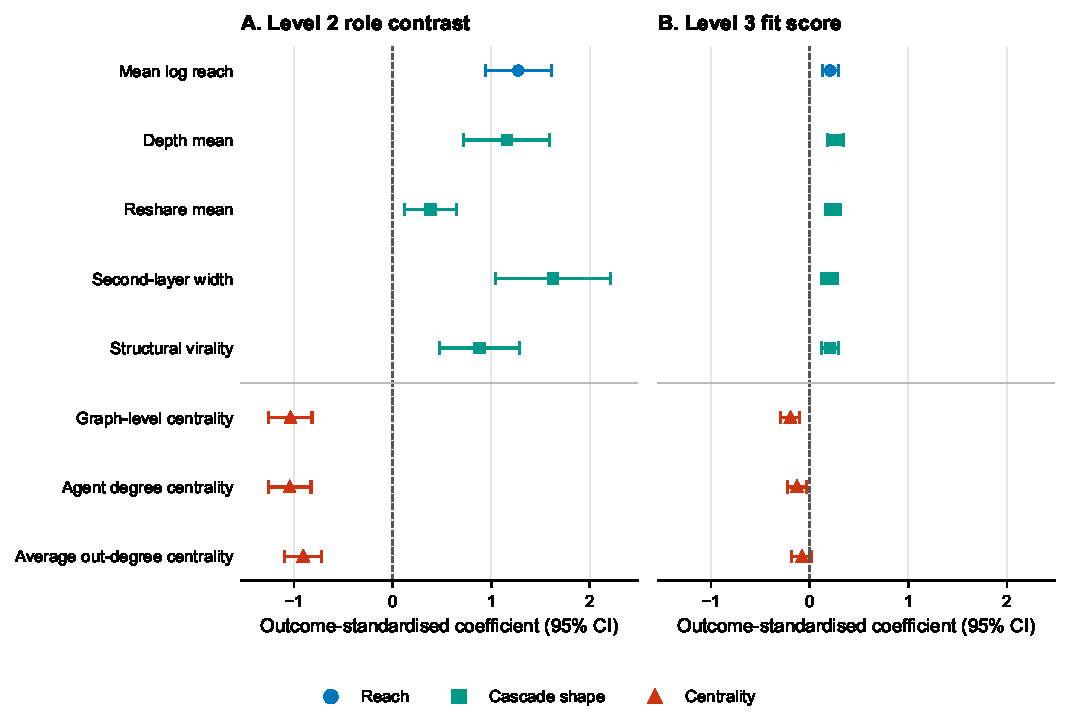
\includegraphics[width=\textwidth]{figures/figure_6_1_reach_centrality_forest.pdf}
\caption{Outcome-standardised coefficients for reach, cascade-shape, and centrality outcomes.}
\label{fig:6-1}
\caption*{Note. Panel A reports the Marketing/Operations contrast relative to Field Sales from the Level 2 core models, with each outcome standardised and controls for agent gender and activity. Panel B reports the \varname{z\_MatchScore\_mean} coefficient from the Level 3 continuous matching specification, with each outcome standardised and the same controls as the main matching model. Horizontal bars show 95\% confidence intervals based on HC3 robust standard errors.}
\end{figure}

\section{Robustness and Sensitivity Results}
\label{sec:6-5-robustness-and-sensitivity-results}

The robustness and sensitivity checks re-estimate each level's core specification under an alternative modelling choice and ask whether that level's main finding persists. The checks are organised by level and focus on the finding most central to each.

\begin{table}[H]
\centering
\small
\caption{Selected robustness and sensitivity checks for the main reach findings}
\label{tab:6-4}
\renewcommand{\arraystretch}{1.15}
\begin{tabularx}{\textwidth}{>{\raggedright\arraybackslash}p{0.36\textwidth}>{\raggedright\arraybackslash}p{0.25\textwidth}>{\raggedright\arraybackslash}X}
\toprule
Level & Check & Key result \\
\midrule
Level 1 & Topic-score model & \varname{z\_CosineSim} = 0.129, p \textless{} 0.001 \\
Level 1 & Topic-PCA model & \varname{z\_CosineSim} = 0.146, p \textless{} 0.001 \\
Level 1 & Distance measures & Euclidean = -0.128; Manhattan = -0.122 \\
Level 1 & Clustered SEs & \varname{z\_CosineSim} remains significant \\
Level 2 & No activity control & Marketing/Operations pattern remains \\
Level 3 & Weighted models & \varname{MatchScore} = 0.191; Match proportion = 0.171 \\
Level 3 & Cells with at least ten cases & \varname{MatchScore} = 1.842; Match proportion = 1.547 \\
Level 3 & Cells with at least thirty cases & Full model not reported \\
\bottomrule
\end{tabularx}
\end{table}

These checks support the same substantive reading as the main models. The Level 1 semantic-consistency association is stable across topic representations, distance measures, and clustered standard errors. The high Level 1 collinearity diagnostic is driven by the alternative distance measures, which are not entered together with \varname{CosineSim} in the main specification. At Level 2, the Marketing/Operations contrasts do not depend on the activity control. At Level 3, the reach association survives exposure weighting and the restriction to agent–topic cells supported by at least ten cases. The thirty-case threshold leaves too few and too concentrated pairs to support the full control specification, so no thirty-case model is reported.
